\documentclass[11pt,a4paper]{article}

\usepackage[a4paper,margin=1in]{geometry}
\usepackage{amsmath,amssymb}
\usepackage{booktabs}
\usepackage{graphicx}
\usepackage{float}
\usepackage{hyperref}
\usepackage{caption}
\usepackage{subcaption}
\usepackage{enumitem}
\usepackage{authblk}
\usepackage{orcidlink}

\graphicspath{{figures/}}
\hypersetup{
  colorlinks=true,
  linkcolor=blue,
  citecolor=blue,
  urlcolor=blue
}

\title{Void-First Formation of Cosmic Filaments and Attractors: An Experimental DRND Test with SDSS, 2M++, and Peculiar-Velocity Data}
\author{Robert K\l{}eczek$^{1}$\,\orcidlink{0009-0009-9774-0446}}
\affil{$^{1}$Independent Researcher}
\date{Version v.1.0.0 -- Draft revised 7 June 2026}

\begin{document}
\maketitle

E-mail: \href{mailto:r.kleczek@advocem.com}{r.kleczek@advocem.com}

\begin{abstract}
We formulate and test a void-first formation concept for the cosmic web. In this picture, cosmic filaments are not treated as primary independent objects seeded only by pre-existing dark-matter ridges. They are instead interpreted as compression ridges formed after the birth and growth of underdense, topologically degraded domains: expanding voids push matter toward their compensation shells, and filaments and attractor nodes arise where two or more such fronts collide or stall. Discrete Relational Network Dynamics (DRND) is used here as an experimental formalism for this chronology, not as an assumed truth. The analysis asks whether present public data contain residual signatures expected from a push-out, void-driven mechanism.

The tests combine: (i) a locked void-lensing amplitude comparison using an SDSS void-lensing profile, (ii) an SDSS DR8 filament-axis orientation test relative to the DRND shell scale $x_{\rm wall}=1.550760$, (iii) a reconstructed 2M++/Carrick velocity-field monopole test with density-environment splitting, and (iv) line-of-sight peculiar-velocity controls from the SDSS Peculiar Velocity catalogue and Cosmicflows-4. The strongest static result is a filament-block radial-axis excess for high shell-score filament points: $\langle |\cos\theta| \rangle=0.54546$ for 8457 equal-weight filament blocks, with a 95 per cent bootstrap interval $[0.54013,0.55075]$ and $p_{\rm boot}<5\times10^{-5}$ against the isotropic expectation $0.5$. The void-lensing amplitude locked by the DRND topological gain $\eta=19/2$ gives $A=0.202936$, within 0.5 per cent of the same-geometry best-fit amplitude $A_{\rm free}=0.203962$, and improves BIC over a zero-signal null by $\Delta{\rm BIC}=74.95$.

The kinematic result is conditional. In the Carrick/2M++ vector field, voids classified operationally as ``void-in-void'' by negative mean outer density at $2.5R_{\rm v}$ show positive monopole outflow at the DRND shell, $\langle v_{\ell=0}\rangle=9.07\,{\rm km\,s^{-1}}$ ($p=0.0277$), rising to $30.06\,{\rm km\,s^{-1}}$ at $2.5R_{\rm v}$ ($p=2.5\times10^{-11}$). The compressed/compensated subsample shows net infall, and line-of-sight PV catalogues do not recover a positive outflow signal under strict geometric filtering. We therefore report a reproducible void-shell radial alignment anomaly and an environment-conditioned vector-field consistency signal for the void-first hypothesis. We do not claim a falsification of $\Lambda$CDM; a decisive comparison requires matched $\Lambda$CDM mocks with the same SDSS selection, void finder, filament finder, and PV/RSD degradation.
\end{abstract}

\section{Conceptual Hypothesis and Scope}

This manuscript is designed as a technical preprint with an accompanying reproducibility package for an experimental cosmological concept: a void-first chronology of filament and attractor formation. The package format is suitable for Zenodo or any comparable research-data repository, but the manuscript is not framed as a publication tied to a particular repository. It does not claim to prove that cosmic filaments are unrelated to gravity or that the standard gravitational-instability picture is already falsified. The sharper statement tested here is:

\begin{quote}
If voids are active topological expulsion domains, then filaments and attractor nodes should retain residual radial memory of matter being pushed from growing void interiors toward compensation shells and collision ridges. The signal should be strongest in void-in-void environments and weakened or reversed where voids are externally compressed.
\end{quote}

The key chronological claim is that a mature filament is a secondary object. It cannot precede the birth of the void domains whose expanding shells create the compression boundary. In this view, an attractor is not only a primordial pull centre; it is also a convergence node where multiple void-driven fronts meet, stall, and concentrate matter.

The central scale used throughout is the DRND shell position
\begin{equation}
x_{\rm wall}=D/R_{\rm v}=1.550760395,
\end{equation}
with shell width
\begin{equation}
\sigma_{\rm wall}=0.577699652.
\end{equation}
This shell is not fitted in the filament or velocity analyses; it is inherited from the preceding DRND compensated-wall search.

The paper reports both positive and negative controls. This is essential because peculiar velocity catalogues are dominated by line-of-sight projection, virial motions, bulk flows, tidal shear, and survey geometry.

\section{Relation to Prior Work and Novelty}

The void-first hypothesis is not presented as if astronomy had never seen active void phenomenology. Several parts of the observational picture already exist in the literature and must be treated as prior art rather than as DRND discoveries.

\paragraph{Void hierarchy and expanding bubbles.}
The excursion-set void hierarchy of Sheth and van de Weygaert introduced the now standard distinction between void-in-void growth and void-in-cloud compression \cite{sheth2004}. In that framework, voids evolve hierarchically, merge, and can squeeze matter into surrounding walls and ridges. Our use of a density split in the Carrick/2M++ field deliberately follows this phenomenological distinction.

\paragraph{Kinematic repellers.}
The Dipole Repeller analysis showed that the Local Group motion can be described using both attraction by overdense regions and an effective repelling contribution associated with a large underdensity \cite{hoffman2017}. This is an important observational precedent: the word ``repeller'' is already meaningful in large-scale-flow analysis. In standard gravity this repulsion is not a new force; it is the dynamical consequence of a missing attraction relative to the surrounding mass distribution.

\paragraph{Topological mapping of the cosmic web.}
Persistent homology, Morse theory and skeleton methods are also established tools in cosmic-web studies. DisPerSE, for example, identifies filaments, walls, clusters and voids through a persistent-topology construction on observed or simulated point sets \cite{sousbie2011}. Thus DRND does not claim novelty merely because it uses graph or topological language.

\paragraph{Discrete spacetime precedents.}
Discrete approaches to quantum gravity, including causal dynamical triangulations, have long studied ensembles of Lorentzian triangulations and observables such as spectral dimension \cite{ambjorn2005}. DRND should therefore be understood as an experimental relational-network formalism being tested against macroscopic data, not as the first attempt to describe spacetime with discrete structures.

The proposed novelty is narrower and more falsifiable. DRND promotes voids from passive underdense regions or map features to phase-degraded relational domains. In the proposed mechanism, a drop in effective connectivity or spectral dimension produces a transport bottleneck, represented by MFPT-like resistance, and this resistance is hypothesized to source a macroscopic shell displacement with the locked topological gain $\eta=19/2$. Filaments and attractors are then interpreted as secondary compression ridges and convergence nodes generated by colliding void-shell fronts. The present paper tests residual consequences of that causal ordering: shell support near $x_{\rm wall}\simeq1.55$, a radial filament-axis memory, and environment-conditioned monopole outflow. The evidence reported below supports these signatures against simple nulls, but it does not by itself prove that a full $\Lambda$CDM simulation cannot generate the same statistics.

\section{Void-First Chronology}

The conceptual timeline differs from the usual bottom-up description of structure growth.

\paragraph{Saturated epoch.}
At early times the relational network is assumed to be close to spectrally saturated, with local spectral dimension $d_s\simeq3$. In this limit, transport is approximately homogeneous and no mature void-shell pressure exists. This is compatible with the near-homogeneity of the CMB, but it is not by itself evidence for DRND.

\paragraph{Graph degradation and void birth.}
As the relational graph degrades, some domains fall below the saturated transport state. In the DRND language these are the first topologically underconnected regions. They behave observationally as nascent voids: regions in which transport delay and phase-space bottlenecking become larger than in the surrounding medium.

\paragraph{Push-out shell formation.}
Matter is displaced from the degraded domain toward an exterior compensation shell. The characteristic shell scale used in this paper is $x_{\rm wall}\simeq1.55$, not the naive void boundary $D/R_{\rm v}=1$. A filament is then interpreted as a ridge on which two or more expanding shells meet, or where a shell is blocked by a neighbouring pressure front.

\paragraph{Attractors as convergence nodes.}
In the void-first view, attractors are not merely pre-existing mass peaks that pull matter in from all directions. They can also be late-time convergence nodes generated where multiple void shells focus and trap displaced matter. This does not remove gravity; it changes the causal ordering being tested.

The observational ``kill switch'' is therefore not the existence of any high-redshift overdensity or short filament-like protostructure. JWST already detects biased high-redshift environments and filamentary structures around quasars, and COSMOS-Web reconstructs large-scale environment to $z\sim7$ \cite{wang2023,hatamnia2026}. The sharper falsification target is the abundance, length scale, and maturity of void-bounded filaments relative to the first detectable voids. A mature, SDSS-like void-and-filament foam appearing before voids have time to form would be damaging for the void-first DRND chronology. Conversely, delayed maturation of void-bounded filaments, with early structures concentrated around biased peaks and protoclusters, remains compatible with the concept. Ly$\alpha$ forest tomography is therefore a natural future test because it can detect high-redshift voids and density/flux structures around $z\simeq2$--3 \cite{krolewski2018,stark2015}.

\section{Early Protostructures Are Not Mature Void-Bounded Filaments}

This distinction is central to the falsifiability of the model. A high-redshift structure called a ``filament'' in the observational literature is not automatically the same object as a late-time, void-bounded cosmic-web filament. We therefore use the following operational distinction.

\paragraph{Local protostructure.}
A local protostructure is a high-redshift overdensity anchored to a biased node such as a luminous quasar, protocluster, or early massive halo. It may contain gas streams, aligned emitters, and filament-like morphology. Its defining feature is that the object is selected around a dense node and need not be bounded on both sides by large, mature voids.

\paragraph{Mature void-bounded filament.}
A mature cosmic-web filament in the void-first DRND sense is a compression ridge between two or more macroscopic void domains. Its defining feature is not simply elongation or galaxy overdensity, but void adjacency: the filament sits near compensation shells and should show shell support relative to neighbouring voids. In the present SDSS test, this is encoded by the shell score around $x_{\rm wall}\simeq1.55$.

The logical consequence is simple. JWST detections of early filamentary structures around quasars do not by themselves falsify void-first DRND. They demonstrate that gravity and local accretion operate in overdense regions at high redshift, which DRND allows in the saturated regime $d_s\simeq3$. What would falsify the chronology is stronger: a statistically mature, globally connected network of thin filaments and large voids at $z>6$, with void sizes and void-bounded morphology comparable to the low-redshift cosmic web.

\begin{table}[H]
\centering
\caption{Operational separation between high-redshift protostructures and the mature void-bounded web required to falsify the void-first chronology.}
\small
\begin{tabular}{p{0.26\linewidth}p{0.40\linewidth}p{0.24\linewidth}}
\toprule
Observation class & Typical evidence & DRND interpretation \\
\midrule
Quasar/protocluster filament at $z\simeq6.6$ & Local overdensity around a biased node \cite{wang2023} & Allowed local accretion \\
COSMOS-Web environments to $z\sim7$ & Density reconstruction; high-$z$ trends strongest in extreme overdensities \cite{hatamnia2026} & Allowed biased early nodes \\
Ly$\alpha$ voids at $z\simeq2.3$ & 3D void detection and void volume fraction \cite{krolewski2018} & Direct void-growth test regime \\
Mature SDSS-like void-and-filament foam at $z>6$ & Large voids plus thin separating ridges over tens of Mpc & Falsifies or strongly damages void-first chronology \\
\bottomrule
\end{tabular}
\normalsize
\end{table}

This gives a restricted proof rather than an absolute proof. The proof is categorical: published JWST protostructures are selected as overdense, biased environments and therefore belong to the local-protostructure class, not automatically to the mature void-bounded-filament class. Since the void-first model permits local overdensities before global void-shell maturation, those observations are not counterexamples. A counterexample must show the mature class at too early a time: large voids and their separating filaments as a global architecture, not merely an overdense string of galaxies near a quasar.

\section{Data}

\subsection{Void Lensing}

The void-lensing input is based on the public SDSS void-lensing measurements associated with Clampitt and Jain's SDSS void analysis \cite{clampitt2015}. The local analysis uses the previously rebinned profile and covariance in the project workspace. The test compares a locked DRND amplitude, a one-parameter same-geometry free amplitude, several fixed physical-amplitude controls, and a zero-signal null.

\subsection{Filament Catalogue}

Filament axes are taken from the SDSS DR8 filament catalogue of Tempel, Stoica and Saar \cite{tempel2014}. The catalogue gives filament spine points and local direction vectors. We convert the catalogue coordinates into the same Cartesian convention used in the void-shell analysis and compare each filament tangent vector with the radial vector from the best-scoring void shell.

\subsection{Peculiar Velocity and Velocity-Field Inputs}

Three kinematic inputs are used.

\begin{enumerate}[leftmargin=1.2cm]
  \item The SDSS Peculiar Velocity catalogue contains 34,059 early-type galaxies with Fundamental Plane distance-ratio information \cite{howlett2022zenodo,howlett2022}.
  \item Cosmicflows-4 provides galaxy and group distances and peculiar velocities \cite{tully2023}. The VizieR group table used here contains 38,053 group entries.
  \item The Carrick et al. 2M++ reconstruction provides a 3D density and peculiar velocity field on a $257^3$ grid in Galactic Cartesian coordinates, spanning $\pm200\,h^{-1}{\rm Mpc}$ \cite{carrick2015}.
\end{enumerate}

The SDSS/eBOSS DR16 RSD product included in the data package is a compressed global BAO/RSD measurement, not a position-by-position velocity catalogue. It is therefore used only as a growth-rate context and not as local evidence for or against void-shell outflow.

\section{Shell and Orientation Statistics}

For each filament spine point $p$ and each void centre $c_i$, define
\begin{equation}
q_i(p)=\frac{|p-c_i|}{R_{{\rm v},i}},
\end{equation}
and the DRND shell score
\begin{equation}
S_i(p)=\exp\left[-\frac{1}{2}\left(\frac{q_i(p)-x_{\rm wall}}{\sigma_{\rm wall}}\right)^2\right].
\end{equation}
The best void for a point is the void maximizing $S_i(p)$. The local filament tangent is $\hat{t}$ and the corresponding radial unit vector is
\begin{equation}
\hat{n}=\frac{p-c_{\rm best}}{|p-c_{\rm best}|}.
\end{equation}
The orientation statistic is
\begin{equation}
T=|\hat{t}\cdot\hat{n}|.
\end{equation}
For isotropic unoriented axes, $\mathbb{E}(T)=0.5$. Because filament spine points are strongly correlated along a single filament, the headline uncertainty is not the point-level uncertainty. We report equal-weight filament-block and void-block statistics with bootstrap intervals.

\begin{table}[H]
\centering
\caption{Main filament-orientation statistics. Bootstrap intervals are block-level equal-weight intervals; the bootstrap lower $p$-value floor is $1/(20000+1)\simeq5\times10^{-5}$.}
\begin{tabular}{lrrrr}
\toprule
Subset & Blocks & Mean $|\cos\theta|$ & 95\% CI & Fraction $>0.5$ \\
\midrule
All filament blocks & 15421 & 0.51450 & [0.51060, 0.51832] & 0.5168 \\
Shell score $>0.5$ & 10270 & 0.53331 & [0.52861, 0.53803] & 0.5465 \\
Shell score $>0.8$ & 8457 & 0.54546 & [0.54013, 0.55075] & 0.5653 \\
Within $0.5\sigma_{\rm wall}$ & 7655 & 0.55490 & [0.54940, 0.56046] & 0.5771 \\
Multi-shell support $\geq2$ & 5756 & 0.52287 & [0.51679, 0.52897] & 0.5412 \\
\bottomrule
\end{tabular}
\end{table}

The radial-axis excess is small in absolute terms, but it survives block weighting. This makes it a robust alignment anomaly rather than a point-count artefact.

\begin{figure}[H]
\centering
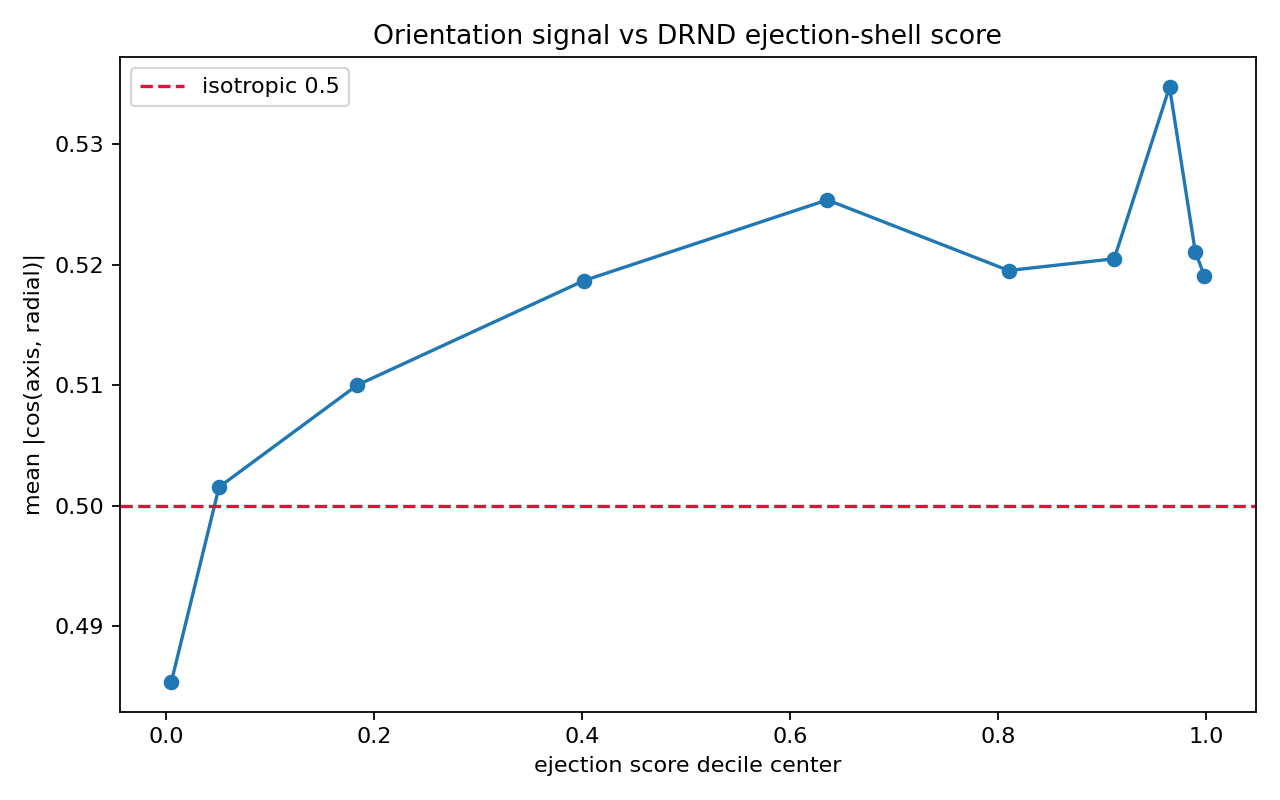
\includegraphics[width=0.88\linewidth]{orientation_deciles.png}
\caption{Mean filament radial-axis statistic $|\cos\theta|$ as a function of DRND shell score decile. The lowest-score decile is below isotropic expectation, while high-score bins are above 0.5. The trend is not perfectly monotonic, which argues against overinterpreting the statistic as a complete dynamical proof.}
\end{figure}

\begin{figure}[H]
\centering
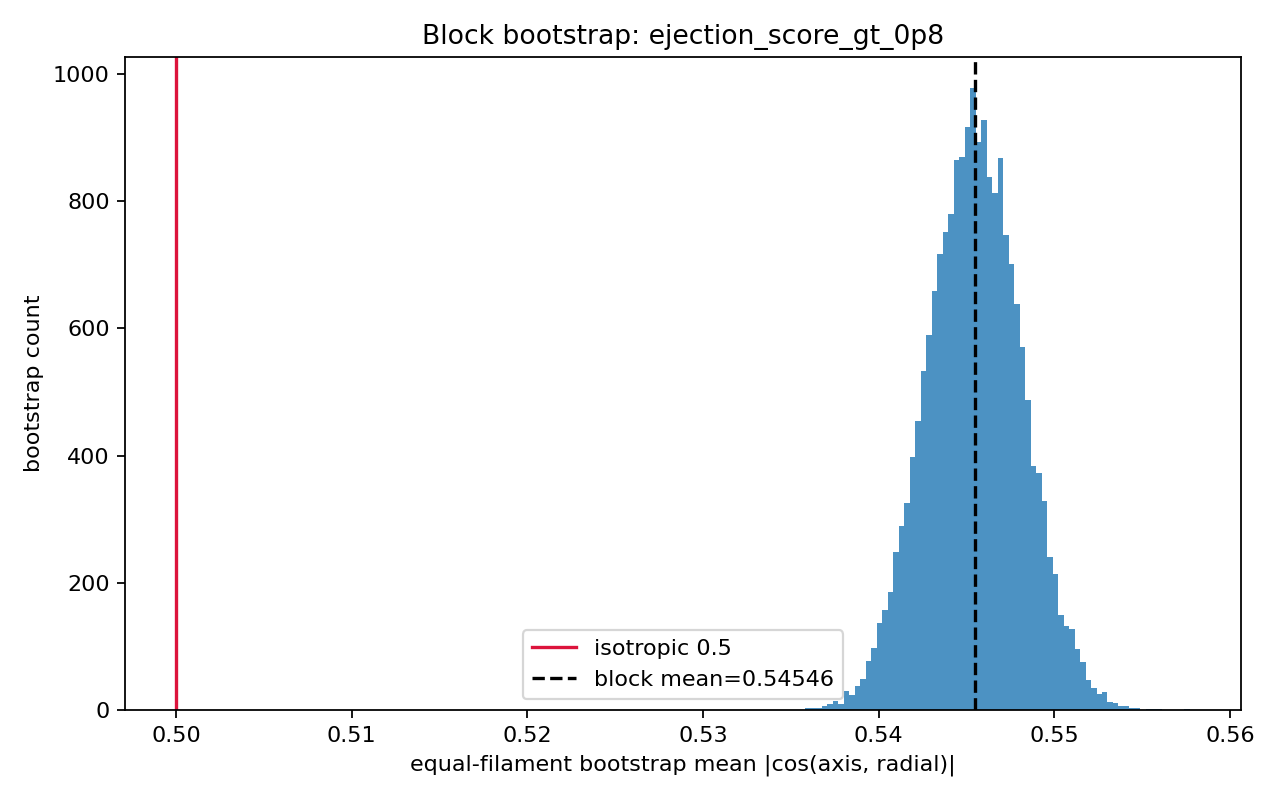
\includegraphics[width=0.76\linewidth]{orientation_bootstrap_score_gt_0p8.png}
\caption{Block-bootstrap distribution for the high shell-score orientation statistic. The filament-block mean is well above the isotropic null expectation of 0.5.}
\end{figure}

\section{Void-Lensing Amplitude Test}

The DRND amplitude test asks whether the same void-lensing geometry can be described by a locked topological gain. The locked gain used here is
\begin{equation}
\eta_{\rm wall}=19/2.
\end{equation}
The corresponding locked amplitude is
\begin{equation}
A_{\rm DRND}=0.202935919,
\end{equation}
while the same-geometry diagnostic free amplitude is
\begin{equation}
A_{\rm free}=0.203962126.
\end{equation}
The locked amplitude is therefore 99.497 per cent of the empirical same-geometry amplitude.

\begin{table}[H]
\centering
\caption{Void-lensing model comparison. Lower BIC is better. The locked DRND amplitude has no fitted amplitude parameter in this comparison.}
\begin{tabular}{lrrrr}
\toprule
Case & $A$ & Parameters & BIC & $\Delta{\rm BIC}$ \\
\midrule
Locked DRND gain $19/2$ & 0.202936 & 0 & 37.70 & 0.00 \\
Free amplitude, same geometry & 0.203962 & 1 & 39.90 & 2.20 \\
Total matter physical-$z$ & 0.137325 & 0 & 45.70 & 8.00 \\
Baryon physical-$z$ & 0.021362 & 0 & 97.77 & 60.07 \\
Zero-signal null & 0.000000 & 0 & 112.65 & 74.95 \\
\bottomrule
\end{tabular}
\end{table}

\begin{figure}[H]
\centering
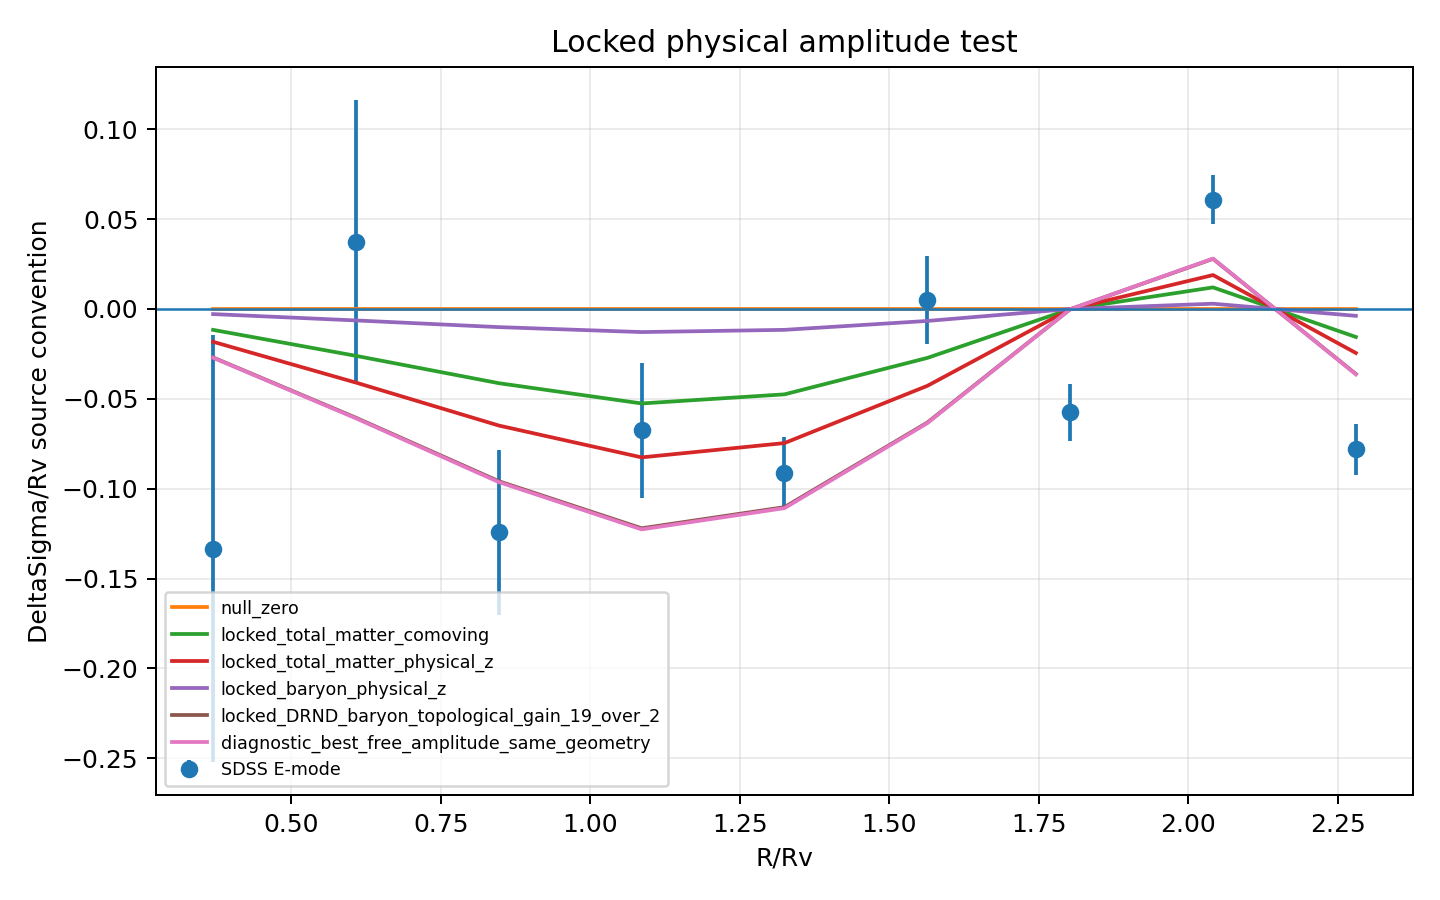
\includegraphics[width=0.86\linewidth]{void_lensing_locked_profile.png}
\caption{Locked DRND void-lensing profile against the rebinned SDSS void-lensing data used in this analysis.}
\end{figure}

\begin{figure}[H]
\centering
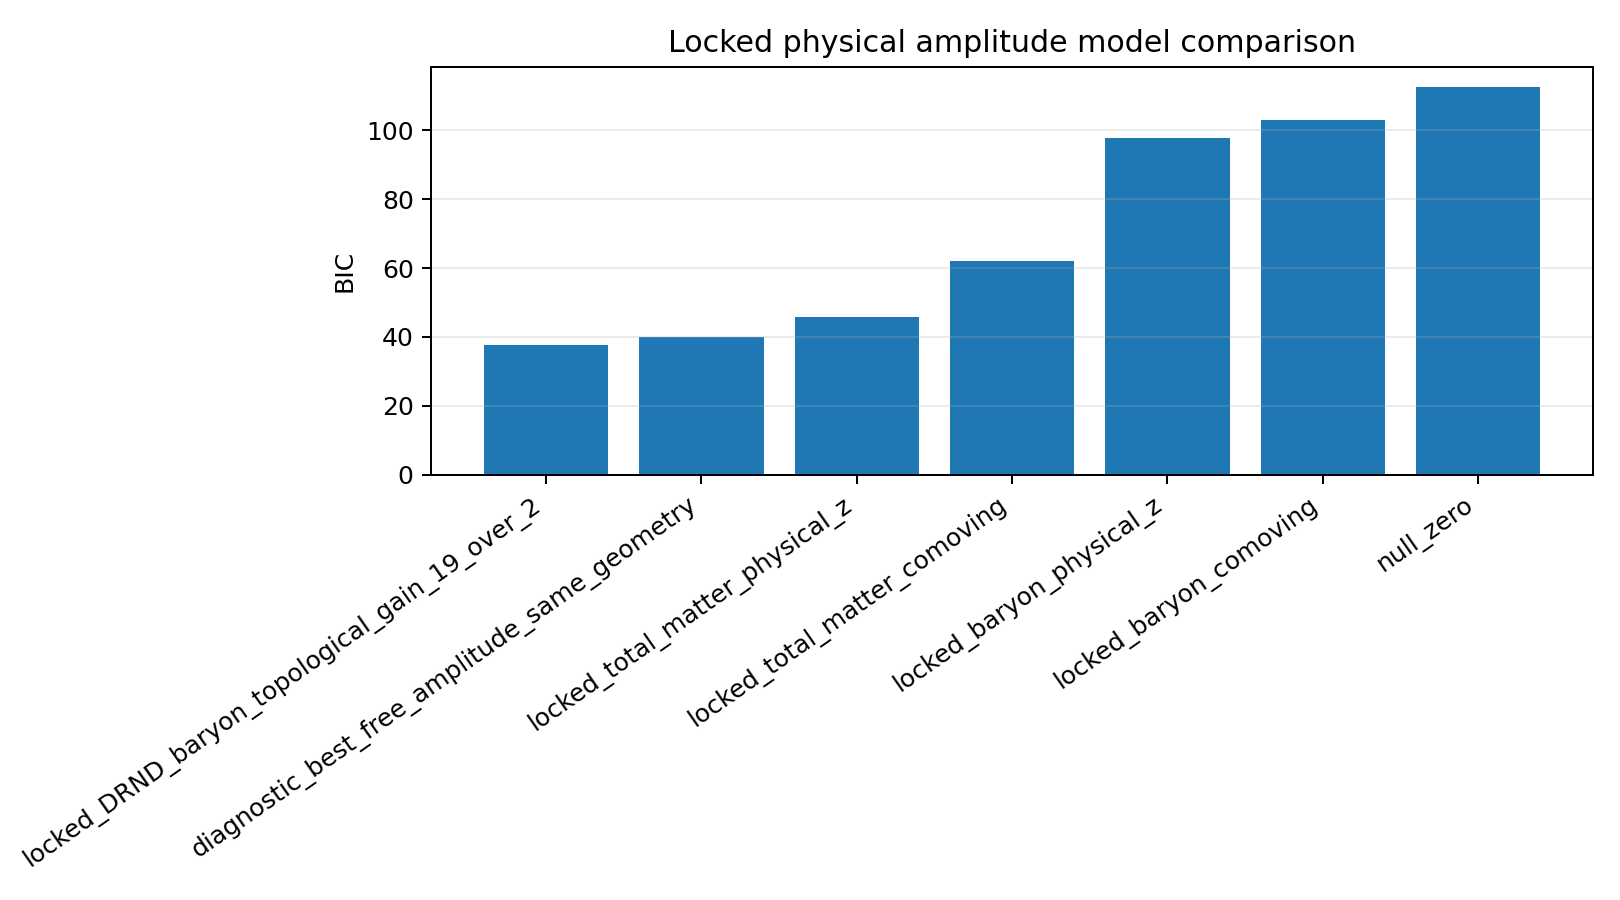
\includegraphics[width=0.78\linewidth]{void_lensing_bic.png}
\caption{BIC comparison for locked and control amplitude models.}
\end{figure}

\section{Velocity-Field Monopole Test}

The Carrick/2M++ vector field allows a genuine 3D velocity test within the local $\pm200\,h^{-1}{\rm Mpc}$ cube. For a void centre $c$ and shell direction $\hat{n}$, define the relative radial velocity
\begin{equation}
v_r(x,\hat{n})=\left[v(c+xR_{\rm v}\hat{n})-v(c)\right]\cdot\hat{n}.
\end{equation}
To separate monopole expansion from dipole bulk flow and quadrupole tidal shear, we fit
\begin{equation}
v_r(\hat{n}) = a_0 + a_x n_x + a_y n_y + a_z n_z + Q(\hat{n}) + \epsilon,
\end{equation}
where $a_0$ is the monopole and $Q(\hat{n})$ is a five-component real quadrupole basis. The reported statistic is $a_0$.

Because not all voids are physically equivalent, we split the 217 Carrick-covered SDSS voids by the mean Carrick luminosity-weighted density contrast at $2.5R_{\rm v}$:
\begin{equation}
\langle \delta_g^\star(2.5R_{\rm v})\rangle < 0 \quad \Rightarrow \quad {\rm void\mbox{-}in\mbox{-}void}.
\end{equation}
The complementary set is labelled compressed/compensated, not as a fundamental taxonomy but as an operational environmental split.

\begin{table}[H]
\centering
\caption{Carrick/2M++ fitted monopole $a_0$ in ${\rm km\,s^{-1}}$. The positive signal appears only after the void-in-void environmental split.}
\begin{tabular}{lrrrr}
\toprule
Shell & Class & $N_{\rm void}$ & Mean $a_0$ & Positive fraction \\
\midrule
$0.8R_{\rm v}$ & void-in-void & 111 & 4.19 & 0.784 \\
$1.0R_{\rm v}$ & void-in-void & 111 & 3.79 & 0.748 \\
$1.25R_{\rm v}$ & void-in-void & 111 & 5.16 & 0.757 \\
$x_{\rm wall}R_{\rm v}$ & void-in-void & 111 & 9.07 & 0.784 \\
$2.0R_{\rm v}$ & void-in-void & 111 & 18.12 & 0.802 \\
$2.5R_{\rm v}$ & void-in-void & 111 & 30.06 & 0.847 \\
\midrule
$x_{\rm wall}R_{\rm v}$ & compressed/compensated & 106 & -64.18 & 0.377 \\
$2.5R_{\rm v}$ & compressed/compensated & 106 & -68.31 & 0.321 \\
\bottomrule
\end{tabular}
\end{table}

At the DRND shell, the void-in-void subsample has $p=0.0277$ for a one-sided test against zero mean monopole. At $2.0R_{\rm v}$ and $2.5R_{\rm v}$ the corresponding $p$-values are $4.7\times10^{-5}$ and $2.5\times10^{-11}$, respectively. The full, unfiltered sample has a negative mean and a near-zero median, showing why a naive all-void average is not physically diagnostic.

\begin{figure}[H]
\centering
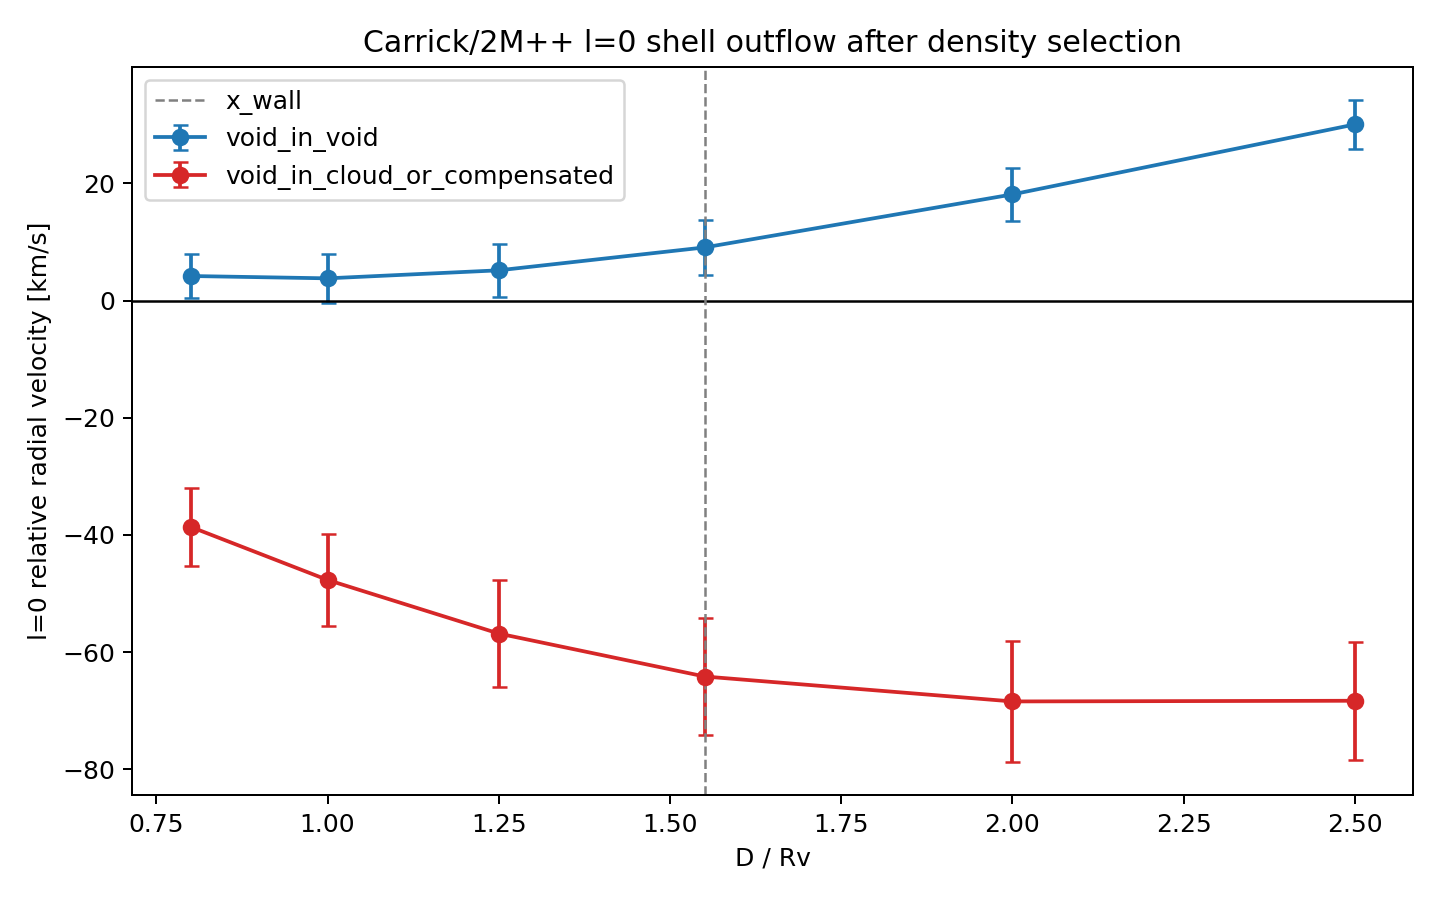
\includegraphics[width=0.90\linewidth]{carrick_l0_profile.png}
\caption{Carrick/2M++ monopole outflow profile after environmental splitting. The void-in-void subsample shows a rising positive monopole, while compressed/compensated voids show net infall.}
\end{figure}

\section{Line-of-Sight Peculiar-Velocity Controls}

For PV catalogues, only the line-of-sight component is observed. We therefore restrict to shell-score $>0.8$ and $|\mu|>0.8$, where
\begin{equation}
\mu=\hat{n}_{\rm void}\cdot\hat{r}_{\rm LOS}.
\end{equation}
The matched radial amplitude estimator is
\begin{equation}
A_{\rm LOS}=\frac{\sum_i v_{{\rm LOS},i}\mu_i}{\sum_i \mu_i^2}.
\end{equation}

The results are negative controls:

\begin{table}[H]
\centering
\caption{Strict LOS PV tests with shell score $>0.8$ and $|\mu|>0.8$.}
\begin{tabular}{lrrrr}
\toprule
Catalogue & Objects & $A_{\rm LOS}$ & Block median & Positive block fraction \\
\midrule
SDSS PV & 1573 & $-191.29$ & $-122.38$ & 0.465 \\
Cosmicflows-4 groups & 1233 & $-123.53$ & $-228.74$ & 0.409 \\
\bottomrule
\end{tabular}
\end{table}

This does not falsify the static alignment result, but it prevents a stronger claim that present LOS PV catalogues independently detect DRND-like void expulsion. The likely contaminants are line-of-sight projection, virial motions, residual group calibration issues, and mismatch between PV selection and the SDSS void/filament volume.

\section{Bayesian Proxies and the Lambda-CDM Control Problem}

We report BIC and approximate Bayes-factor proxies using
\begin{equation}
\log_{10}B_{10}\simeq\frac{\Delta{\rm BIC}}{2\ln 10},
\end{equation}
where positive values favour the alternative over the stated null. These numbers are useful ranking diagnostics, not a final DRND-versus-$\Lambda$CDM evidence ratio.

\begin{table}[H]
\centering
\caption{Bayesian proxy summary. ``Free mean'' alternatives test for an empirical anomaly relative to a fixed null; they are not full generative DRND likelihoods.}
\begin{tabular}{lrrr}
\toprule
Test & $N$ & $\Delta{\rm BIC}$ & $\log_{10}B$ proxy \\
\midrule
Void-lensing locked DRND vs zero null & 9 & 74.95 & 16.27 \\
Void-lensing locked DRND vs free same geometry & 9 & 2.20 & 0.48 \\
Filament orientation, shell score $>0.8$, free mean vs 0.5 & 8457 & 270.82 & 58.81 \\
Carrick void-in-void, $x_{\rm wall}$, free mean vs 0 & 111 & -0.99 & -0.21 \\
Carrick void-in-void, $2.0R_{\rm v}$, free mean vs 0 & 111 & 10.74 & 2.33 \\
Carrick void-in-void, $2.5R_{\rm v}$, free mean vs 0 & 111 & 39.07 & 8.48 \\
\bottomrule
\end{tabular}
\end{table}

The strongest model-selection numbers come from void lensing and filament orientation. The Carrick velocity-field result becomes model-selection positive only outside the exact DRND shell, where the void-in-void monopole grows. This is physically suggestive but should be treated as a conditional kinematic consistency signal, not as decisive evidence.

A rigorous comparison to classical $\Lambda$CDM requires:
\begin{enumerate}[leftmargin=1.2cm]
  \item matched $\Lambda$CDM mock catalogues with the same SDSS angular mask, redshift limits, void finder and filament finder;
  \item the same shell-score statistic applied blindly to mocks;
  \item mock PV and RSD reconstructions degraded to the same observational selection and distance errors;
  \item a pre-registered likelihood comparing a topological-ejection shell model with a collapse-only or simulation-calibrated $\Lambda$CDM null.
\end{enumerate}

Until those mocks are run, the safest statement is: the data show a statistically robust void-shell radial orientation anomaly and an environment-conditioned vector-field outflow signature that are compatible with the void-first DRND concept and not captured by a simple isotropic null. They do not yet establish that the same effect is absent in a fully realistic $\Lambda$CDM realization.

\section{Limitations}

\begin{itemize}[leftmargin=1.2cm]
  \item The filament orientation signal is statistically strong but small in absolute amplitude.
  \item The SDSS galaxy null is not a pure noise null because galaxies themselves live in the cosmic web.
  \item The Carrick/2M++ field is a reconstructed velocity field derived from a density model; it is not an independent direct PV catalogue.
  \item The SDSS PV conversion used here is a quick low-redshift line-of-sight proxy based on log-distance-ratio quantities. A final PV likelihood should fit the catalogue observable directly.
  \item The Cosmicflows-4 and SDSS PV LOS tests are negative under the present geometric filter.
  \item JWST detections of high-redshift biased structures and filamentary protostructures mean the void-first hypothesis cannot be stated as ``no early filaments at all''. The falsifiable claim is instead about the delayed emergence of mature, void-bounded filament and attractor architecture.
  \item No claim is made that $\Lambda$CDM is falsified. The present comparison is against isotropic, shuffled and amplitude nulls, plus a reconstructed-field environmental split.
\end{itemize}

\section{Reproducibility Package}

The accompanying archival reproducibility package contains:
\begin{itemize}[leftmargin=1.2cm]
  \item the LaTeX source and compiled PDF;
  \item processed evidence tables for void lensing, filament orientation, velocity-field dynamics and Bayes proxies;
  \item figures used in this manuscript;
  \item scripts used to audit PV inputs and run the refined velocity analysis;
  \item a data-source manifest pointing to the raw public catalogues.
\end{itemize}

\section{Conclusion}

The present analysis supports a cautious but nontrivial version of the void-first concept. The SDSS filament catalogue shows a robust radial-axis excess relative to the compensated void shell. The SDSS void-lensing profile is consistent with the locked DRND topological gain amplitude. The Carrick/2M++ vector field shows positive monopole outflow only after selecting void-in-void environments, while compressed/compensated voids show infall. Direct LOS PV catalogues do not recover a positive signal.

The resulting picture is not a proof that gravity or dark-matter structure is irrelevant. It is a falsifiable alternative chronology: voids are treated as active transport-degraded domains; filaments are secondary compression ridges produced by colliding void-shell fronts; attractors are convergence nodes where several such fronts stall and concentrate matter. In this chronology the present data support the existence of a radial memory at the shell, but they also show that external compression and LOS observational geometry can erase or reverse the kinematic signal.

The evidence is strong enough to justify a public preprint and reproducibility release as an experimental DRND test of filament and attractor formation. The decisive next step is a matched $\Lambda$CDM mock comparison and a direct likelihood treatment of PV observables. If mature void-bounded filament networks appear in simulations and observations before void domains can form, the void-first chronology is falsified. If the shell-alignment and void-in-void outflow signatures persist under matched mocks and high-redshift tomography, the concept becomes a viable competing formation channel for the cosmic web.

\begin{thebibliography}{17}

\bibitem{ambjorn2005}
Ambjorn, J., Jurkiewicz, J., \& Loll, R. 2005,
``Spectral dimension of the universe,''
\emph{Physical Review Letters}, 95, 171301.
doi: \href{https://doi.org/10.1103/PhysRevLett.95.171301}{10.1103/PhysRevLett.95.171301}.

\bibitem{carrick2015}
Carrick, J., Turnbull, S. J., Lavaux, G., \& Hudson, M. J. 2015,
``Cosmological parameters from the comparison of peculiar velocities with predictions from the 2M++ density field,''
\emph{Monthly Notices of the Royal Astronomical Society}, 450, 317--332.
doi: \href{https://doi.org/10.1093/mnras/stv547}{10.1093/mnras/stv547}.

\bibitem{clampitt2015}
Clampitt, J., \& Jain, B. 2015,
``Lensing measurements of the mass distribution in SDSS voids,''
\emph{Monthly Notices of the Royal Astronomical Society}, 454, 3357--3365.
doi: \href{https://doi.org/10.1093/mnras/stv2215}{10.1093/mnras/stv2215}.

\bibitem{howlett2022zenodo}
Howlett, C. et al. 2022,
``The SDSS Peculiar Velocity Catalogue,''
Zenodo data release.
doi: \href{https://doi.org/10.5281/zenodo.6824749}{10.5281/zenodo.6824749}.

\bibitem{hatamnia2026}
Hatamnia, H., Mobasher, B., Taamoli, S., et al. 2026,
``Large-scale Structure in COSMOS-Web: Tracing Galaxy Evolution in the Cosmic Web up to $z\sim7$ with the Largest JWST Survey,''
\emph{The Astrophysical Journal}, 1002, 192.
doi: \href{https://doi.org/10.3847/1538-4357/ae5bac}{10.3847/1538-4357/ae5bac}.

\bibitem{howlett2022}
Howlett, C., Said, K., Lucey, J. R., et al. 2022,
``The Sloan Digital Sky Survey Peculiar Velocity Catalogue,''
arXiv: \href{https://arxiv.org/abs/2201.03112}{2201.03112}.

\bibitem{hoffman2017}
Hoffman, Y., Pomarede, D., Tully, R. B., \& Courtois, H. M. 2017,
``The Dipole Repeller,''
\emph{Nature Astronomy}, 1, 0036.
doi: \href{https://doi.org/10.1038/s41550-016-0036}{10.1038/s41550-016-0036}.

\bibitem{krolewski2018}
Krolewski, A., Lee, K.-G., White, M., Hennawi, J. F., et al. 2018,
``A Detection of $z\sim2.3$ Cosmic Voids from 3D Lyman-$\alpha$ Forest Tomography in the COSMOS Field,''
\emph{The Astrophysical Journal}.
doi: \href{https://doi.org/10.3847/1538-4357/aac829}{10.3847/1538-4357/aac829}.

\bibitem{sheth2004}
Sheth, R. K., \& van de Weygaert, R. 2004,
``A hierarchy of voids: much ado about nothing,''
\emph{Monthly Notices of the Royal Astronomical Society}, 350, 517--538.
doi: \href{https://doi.org/10.1111/j.1365-2966.2004.07661.x}{10.1111/j.1365-2966.2004.07661.x}.

\bibitem{sousbie2011}
Sousbie, T. 2011,
``The persistent cosmic web and its filamentary structure -- I. Theory and implementation,''
\emph{Monthly Notices of the Royal Astronomical Society}, 414, 350--383.
doi: \href{https://doi.org/10.1111/j.1365-2966.2011.18394.x}{10.1111/j.1365-2966.2011.18394.x}.

\bibitem{stark2015}
Stark, C. W., Font-Ribera, A., White, M., \& Lee, K.-G. 2015,
``Finding high-redshift voids using Lyman $\alpha$ forest tomography,''
\emph{Monthly Notices of the Royal Astronomical Society}, 453, 4311--4323.
doi: \href{https://doi.org/10.1093/mnras/stv1868}{10.1093/mnras/stv1868}.

\bibitem{tempel2014}
Tempel, E., Stoica, R. S., \& Saar, E. 2014,
``Detecting filamentary pattern in the cosmic web: a catalogue of filaments for the SDSS,''
\emph{Monthly Notices of the Royal Astronomical Society}, 438, 3465--3482.
doi: \href{https://doi.org/10.1093/mnras/stt2454}{10.1093/mnras/stt2454}.

\bibitem{tully2023}
Tully, R. B., Kourkchi, E., Courtois, H. M., et al. 2023,
``Cosmicflows-4,''
\emph{The Astrophysical Journal}, 944, 94.
doi: \href{https://doi.org/10.3847/1538-4357/ac94d8}{10.3847/1538-4357/ac94d8}.

\bibitem{wang2023}
Wang, F., Yang, J., Hennawi, J. F., et al. 2023,
``A SPectroscopic Survey of Biased Halos in the Reionization Era (ASPIRE): JWST Reveals a Filamentary Structure around a $z=6.61$ Quasar,''
\emph{The Astrophysical Journal Letters}, 951, L4.
doi: \href{https://doi.org/10.3847/2041-8213/accd6f}{10.3847/2041-8213/accd6f}.

\bibitem{zeldovich1970}
Zel'dovich, Ya. B. 1970,
``Gravitational instability: An approximate theory for large density perturbations,''
\emph{Astronomy and Astrophysics}, 5, 84--89.

\end{thebibliography}

\end{document}
